\documentclass[11pt]{article}

\usepackage{amsmath}
\usepackage{textcomp}
\usepackage[top=0.8in, bottom=0.8in, left=0.8in, right=0.8in]{geometry}
% Add other packages here %
\usepackage[skip=.4\baselineskip]{parskip}
\usepackage{graphicx}
\usepackage{wrapfig}
\usepackage{lipsum}
\usepackage{subcaption}
\usepackage{enumitem}

% Put your group number and names in the author field %
\title{\bf Exercise 1.\\ Implementing a first Application in RePast: A Rabbits Grass Simulation.}
\author{Group \textnumero 22: Dubuis Samuel, Facklam Oliver}

\begin{document}
\maketitle

\section{Implementation}
After having followed the tutorials of John T. Murphy from the University of Arizona, we ended up with a working simulation of the rabbits in grass scenario.
Throughout the coding, we had to make a few assumptions that we will now describe. We will also talk about particular remarks on our implementation.

\subsection{Assumptions}
% Describe the assumptions of your world model and implementation (e.g. is the grass amount bounded in each cell) %

Most of our assumptions are situated in the schedule part of the simulation. The first one we made is about the grass that the rabbits eat. We decided that at every step, when repopulating the space with grass based on the \texttt{GrassGrowthRate} value, each unit of grass is uniformly distributed, which means that a cell can get multiple units of grass. However we limited the grass to a maximum of 15 per spot. If some grass spawns on a full cell, that unit of grass is lost.

We also assumed that each unit of grass provides one unit of energy to the consuming rabbit. So when a rabbit lands on a particular cell, instead of only gaining one energy, it would gain energy equal to the amount of grass that spawned at this space. If a rabbit cannot move due to a collision, and grass spawned at that exact location, it would eat the grass.

The last assumption is about energy consumption. Reproducing consumes \texttt{birthThreshold} units of energy of the parent rabbit, leaving its energy after reproduction close to 0. Every move costs one energy.

\subsection{Implementation Remarks}
% Provide important details about your implementation, such as handling of boundary conditions %
A couple particular implementation remarks are to be noted.

First is the death of the rabbit when its energy reaches 0. In the tutorial of John Murphy, when an agent's steps to live get below 10, it changes color, and when it dies, it disappears from the grid and is added to the count of dead agents. In our implementation we skipped the changing color part, and also we are not counting how many rabbits died.

Also, when displaying the grass on the grid, the square starts as quite dark, though of the color green. The closer it gets to the max value of 15, the brighter green the square becomes. To display this, we implemented a \texttt{ColorMap} that maps the value at the particular spot on the grid to a shade of green.

To allow rabbits to not bump into the edge of the grid, the space is actually considered to be a torus.
Also, moving-wise, we implemented a switch for the rabbit's movement so it can only move to the cardinal directions, being North, East, South and West.

Reproduction of rabbits is executed at the end of every simulation step. The existing rabbits that have enough energy in that moment create a new rabbit and lose some of their energy.

We also made sure that the list of agents in our simulation wouldn't get bigger than the number of possible agents in our grid, as this number is limited by the \texttt{gridSize}.

\section{Results}
% In this section, you study and describe how different variables (e.g. birth threshold, grass growth rate etc.) or combinations of variables influence the results. Different experiments with diffrent settings are described below with your observations and analysis
In this section we will describe a few experiments that we made based on our working simulation. The main parameters we modified are the \texttt{GrassGrowthRate} and \texttt{BirthThreshold}.
We kept \texttt{GridSize} at 20.

\subsection{Experiment 1}
\begin{figure}[h!]
    \begin{subfigure}{.5\textwidth}
        \centering
        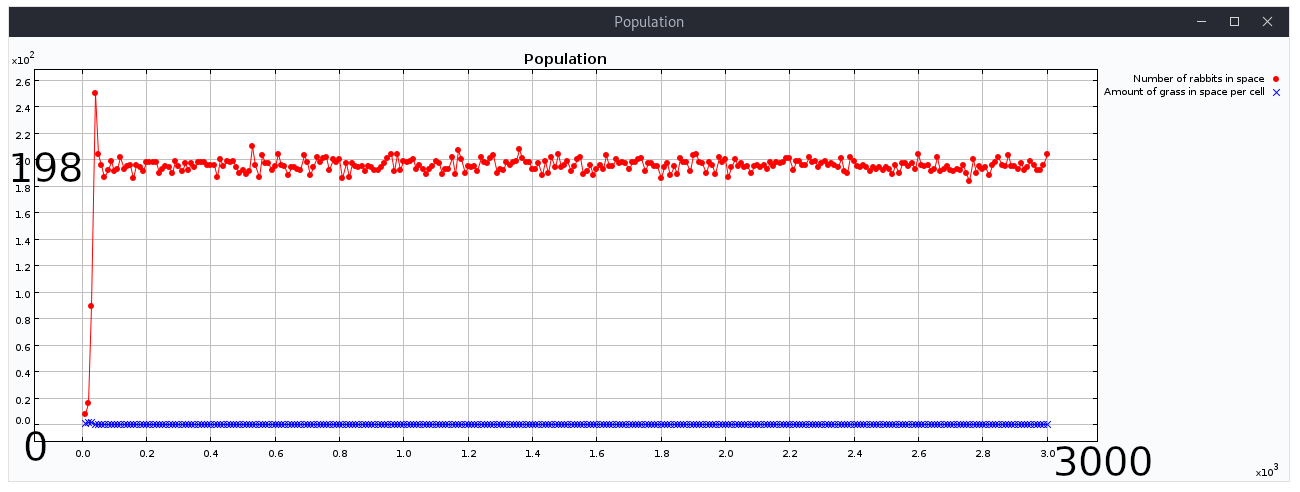
\includegraphics[width=.95\linewidth]{intro_rabbits/plot15_50.png}
        \caption{\texttt{BirthThreshold} 15; \texttt{GrassGrowthRate} 50}
        \label{fig:plot15-50}
    \end{subfigure}
    \hfill
    \begin{subfigure}{.5\textwidth}
        \centering
        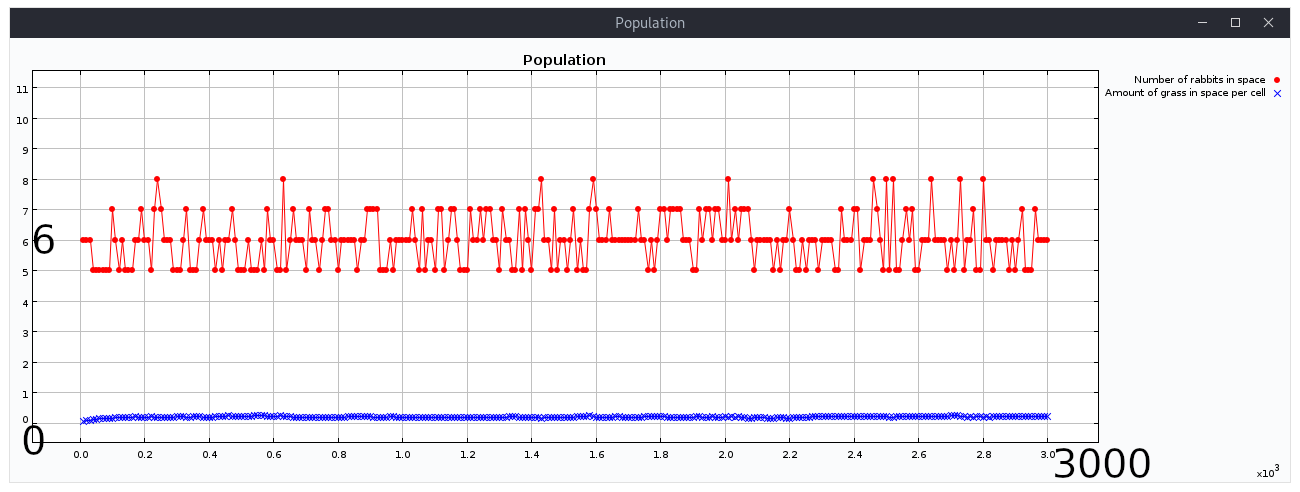
\includegraphics[width=.95\linewidth]{intro_rabbits/plot15_1.png}
        \caption{\texttt{BirthThreshold} 15; \texttt{GrassGrowthRate} 1}
        \label{fig:plot15-1}
    \end{subfigure}\\%
    \begin{subfigure}{.5\textwidth}
        \centering
        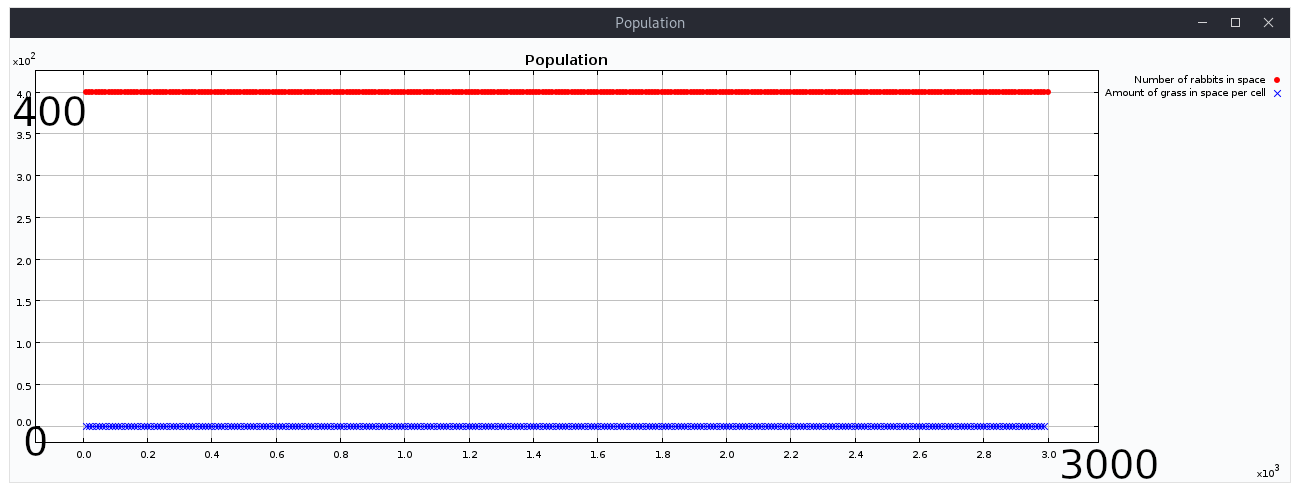
\includegraphics[width=.95\linewidth]{intro_rabbits/plot2_1.png}
        \caption{\texttt{BirthThreshold} 2; \texttt{GrassGrowthRate} 50}
        \label{fig:plot2-50}
    \end{subfigure}
    \hfill
    \begin{subfigure}{.5\textwidth}
        \centering
        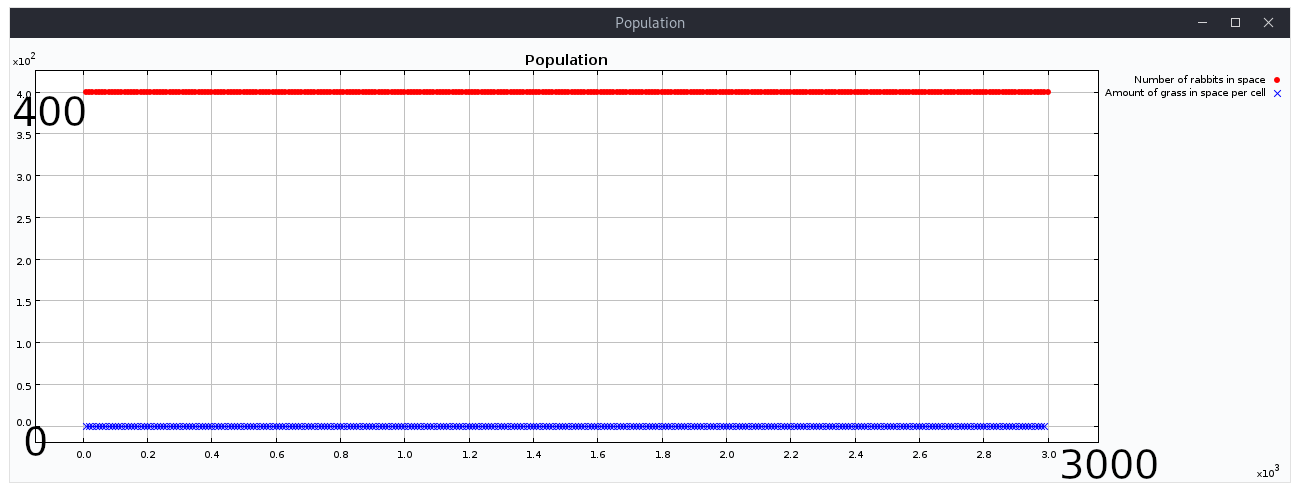
\includegraphics[width=.95\linewidth]{intro_rabbits/plot2_1.png}
        \caption{\texttt{BirthThreshold} 2; \texttt{GrassGrowthRate} 1}
        \label{fig:plot2-1}
    \end{subfigure}%\\%
    \caption{Plots of rabbit count (red) and grass/cell (blue) at each step, for different parameter settings}
    \label{fig:exp1}
\end{figure}

\subsubsection{Setting}
In this first experiment, we start with a single rabbit at 20 life steps and 20 initial grass.  We execute 4 runs of our simulation to compare the impact on rabbit population of:
\begin{itemize}[nosep]
    \item a \texttt{BirthThreshold} which can be high (15) or low (2)
    \item a \texttt{GrassGrowthRate} which can be high (50) or low (1)
\end{itemize}

\subsubsection{Observations}
% Elaborate on the observed results %

The situation with a high birth threshold and high grass growth is shown in figure (\ref{fig:plot15-50}). We get an average of about 198 rabbits alive at the same time. As seen on the plot, at the start the rabbit count immediately increases as each born rabbit gives birth to a new one, then it stabilizes. The large \texttt{GrassGrowthRate} allows the rabbits to reproduce multiple times. If there had been a higher \texttt{GrassGrowthRate}, the grid would probably have filled completely as each rabbit could have gained more energy to rebirth multiple times.

In the second situation, presented in figure (\ref{fig:plot15-1}), the grass growth rate is reduced to a very low number, so that rabbits definitely need to look for source of energy. 
We can see that the first few rabbits give birth immediately as they spawn, having enough energy, but then die when their energy is depleted. Since grass is rare, none of them can find enough source of energy to reproduce another time. Logically, the average is around 6 rabbits, which is the number of rabbits that can be spawned before the first one dies.

The third situation combines a high grass growth rate with a low birth threshold, and is shown in figure (\ref{fig:plot2-50}). We can predict that with a small birth threshold, rabbits will birth multiples times in the same simulation, and with enough grass, the grid will become full. This is exactly what we observe: the grid fills in an instant and stays that way; as soon as a rabbit dies, another one replaces it.

In the last situation, shown in figure (\ref{fig:plot2-1}), both parameters are set to low values. We can predict that the number of rabbits will be higher than in situation 2 since the birth threshold is lower; however there is close to no grass to enable additional reproduction.
Despite this lack of grass, there are enough of them so that the grid fills up instantaneously. 

\begin{figure}[h!]
    \begin{subfigure}{.5\textwidth}
        \centering
        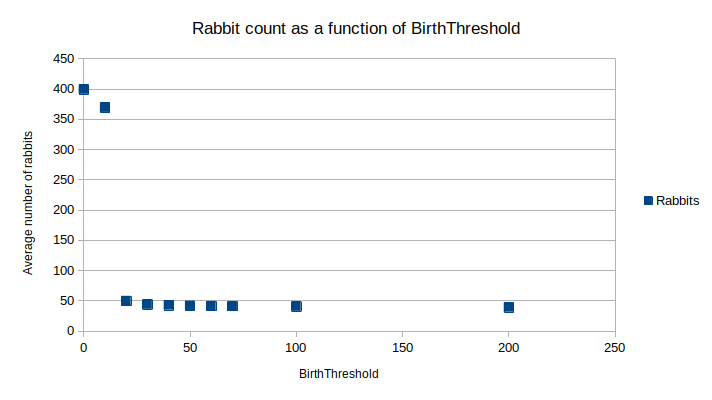
\includegraphics[width=.95\linewidth]{intro_rabbits/birththreshold.png}
        \caption{Average number of rabbits vs. birth threshold}
        \label{fig:birththreshold}
    \end{subfigure}
    \hfill
    \begin{subfigure}{.5\textwidth}
        \centering
        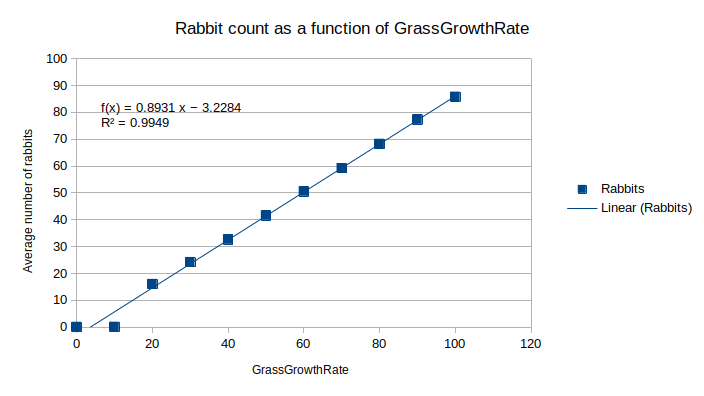
\includegraphics[width=.95\linewidth]{intro_rabbits/grassgrowthrate.png}
        \caption{Average number of rabbits vs. grass growth rate}
        \label{fig:grassgrowthrate}
    \end{subfigure}
    \caption{Plots for experiments 2 \& 3}
    \label{fig:my_label}
\end{figure}

\subsection{Experiment 2}
\subsubsection{Setting}
In the second experiment, we want to analyze how the average rabbit count depends on the birth threshold. For this, we fix \texttt{GrassGrowthRate} to 50, and start with 10 rabbits, 20 initial energy and 0 grass. We then vary the \texttt{BirthThreshold} and for each value we plot the number of rabbits averaged over time. Results are shown in figure (\ref{fig:birththreshold}).

\subsubsection{Observations}

When the birth threshold is below the rabbits' initial energy (20), the grid has a tendency to fill up very quickly: the average number of rabbits is more than 350. However, when the birth threshold is higher than the initial energy, this threshold value doesn't seem to significantly influence the rabbit count.

\subsection{Experiment 3}
\subsubsection{Setting}
In this last experiment, we analyze the relationship between average rabbit count and grass growth. We use the same initial values as in the previous experiment and fix \texttt{BirthThreshold} to 50. We then vary the \texttt{GrassGrowthRate}. Results are shown in figure (\ref{fig:grassgrowthrate}). 

\subsubsection{Observations}

Apart from the first couple of points which represent extreme situations, we observe a strong linear relationship between rabbit count and grass growth rate. The slope is 0.89 and the intercept -3.23.

% I don't think we should add any sections (a TA said so), and a conclusion wasn't in the template (even though it's weird)
%\section{Conclusion}
%As seen in all of the experiments, it seems that setting a \texttt{BirthThreshold} to a low value shows no valuable information. When too low, the rabbits are able to reproduce too often, filling up the grid rapidly. We could experiment further with a bigger grid to maybe see differences, but this is content for another time.
\end{document}